\documentclass[12pt,a4paper]{article}
\usepackage[utf8]{inputenc}
\usepackage{amsmath}
\usepackage{amsfonts}
\usepackage{amssymb}

%bold Greek letters and other symbols
\usepackage{bm}
\usepackage{graphics}
\usepackage[T1]{fontenc}
\usepackage[english]{babel}
\usepackage{graphicx}
\usepackage[left=2.5cm,right=3.0cm,top=2.5cm,bottom=3cm]{geometry}
\usepackage{color}
%
\usepackage{makeidx}
\usepackage{shortvrb,latexsym}

\setlength{\parindent}{0pt}
%\renewcommand{\floatpagefraction}{.99}
%\renewcommand{\textfraction}{.01}
\def \uu  {\bm{u}}
\def \oo {\bm{\omega}}
\def \curl {\bm{\nabla}\times}
\def \dive {\bm{\nabla}\cdot}
\newcommand{\bu}{\bm{u}}
\newcommand{\bv}{\bm{v}}
\newcommand{\rd}{\mathrm{d}}
\newcommand{\hx}{{\bf\hat{x}}}
\newcommand{\hy}{{\bf\hat{y}}}
\newcommand{\hz}{{\bf\hat{z}}}
\newcommand{\hr}{{\bf\hat{r}}}
\newcommand{\hn}{{\bf\hat{n}}}

\begin{document}

\begin{center}
2020-06-16
\end{center}
STOCKHOLMS UNIVERSITET\\
Meteorologiska Institutionen\\
Jonas Nycander, Dhrubaditra Mitra\\
\vspace{1cm}

\begin{center}
{\bf\large Exam in Fluid mechanics (MO5001)}\\
\end{center}

Write the solution of each problem on a separate paper, and write your identification number on every paper.\\

{\bf Allowed aids:} calculator, sheet with vector analysis relations.\\

{\bf Grading:} A 90-100\%, B 80-89\%, C 65-79\%, D 55-64\%, E 50-54\%, Fx 45-49\%, F 0-44\% \\
\vspace{0.5cm}

\begin{enumerate}

\item \label{prb1} Answer the following short questions. You just need to write the final answer. Each question is worth 3 points. 
  \begin{enumerate}
  \item A vector field, $\bu$, with components $u_x$, $u_y$ and $u_z$,  as a function  of
    space (described by $x$, $y$, and $z$ coordinates )
    is give by the following expression
    \begin{eqnarray}
      u_x &=& \cos(y) + 5z^3 ] \nonumber \\
      u_y &=& \alpha[ \exp(-\cosh(x)) ] \nonumber \\
      u_z &=& \alpha[ \sin(x) -y ]
    \end{eqnarray}
   Calculate $\dive \uu$. 
 \item A velocity field $\bu$ in two-dimensions $(x,y)$ is given by the following expression
   \begin{subequations}
     \begin{align}
     u_x &= -x + Sy \\
     u_y &= y  \/.
     \end{align}
     \label{eq:uu}
   \end{subequations}
   Calculate the gradient matrix $ G_{\alpha\beta} \equiv \partial_{\beta}u_{\alpha}$, where
   $\partial_{\beta}$ denote spatial derivative, as a function of $x$ and $y$. Is this velocity
   field incompressible ? 
 \item From Eq.~\ref{eq:uu}  calculate vorticity and rate-of-strain as a function of
   space coordinates, $x,y$.
  \item In which of the following cases can I write the velocity $\vec{v} = \nabla \Psi $ where $\Psi$ is a scalar function
    without any loss of generality: \\
    (a) if the flow is incompressible, (b) if the flow is irrotational, or (c) if the flow is steady.
  \item The lubrication approximation, equations that describes a laminar boundary layer, 
and the
    shallow-water equations are all derived
    from the incompressible Navier--Stokes equations.
The first two assumes that the Reynolds number is small. The third one does not. 
However, they all have a crucial common aspect. What is it ?   
    \end{enumerate}

\item \label{prb3} A thin rectangular plate of dimension $L_x\times L_z$ 
is immersed in a fluid  of
kinematic viscosity $\nu$ and density $\rho$. The plate is being
pulled by a force such that it moves with a velocity $v$ along the $x$
direction. Far away from the plate the fluid is at rest. Assume that the flow is
  laminar. Ignore the edge effects. 
  Estimate the the power necessary to keep the plate moving with a constant velocity.
    (Hint : The power necessary
    is equal to the power dissipated by the viscous forces. You can estimate the
    viscous forces from the stress at the surface of the disc. You need the thickness
    of the boundary layer to estimate the stress. ) (5p)

\item \label{prb4} Same as in Problem~\ref{prb3} with an additional feature:
  the plate is confined vertically within a cavity. The clearance between the
  disk and the horizontal planes of the cavity is equal to $h$ where $h \ll L_x $
  and $h \ll L_y$  as shown in figure~\ref{pipe_disc}.
   Ignore the edge effects. 
  Calculate  the the power necessary to keep the plate moving. 
    (Hint : Use lubrication approximation )  (5p)

  \begin{figure}
    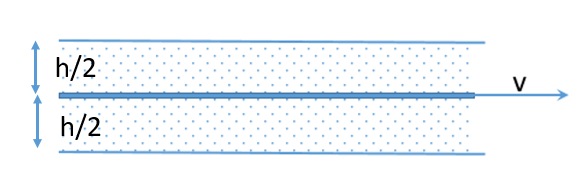
\includegraphics[width=0.4\linewidth]{plate.png}
    \caption{\label{pipe_disc} Problem \ref{prb4} }
  \end{figure}
  %===================================================================

%====================================================================
\end{enumerate}
\end{document}
